          \section{Modelle}
Im folgenden Teil werden die entwickelten Deep Learning Modelle vorgestellt. Für jedes Modell ist der grundlegende Ablauf derselbe (siehe Abbildung \ref{img:workflow}). Die Aufnahme wird vorab auf die Länge 5s zugeschnitten. Anschliessend wird ein Spektrogramm generiert. Die Werte des Spektrogramms werden in die Dezibell Skala umgerechnet und dann normiert. Die Grösse des Spektrogramms unterscheidet sich zwischen den Modellen. Schliesslich berechnet ein Neuronales Netzwerk aus dem Spektogramm eine Vorhersage für die drei Sprachen. 
\\
Insgesamt werden drei grundsätzlich verschiedene Neuronalen Netzwerk Architekturen vorgestellt. Die ersten zwei Modelle sind Convolutional Neural Networks während das dritte Modell eine Kombination zwischen CNN und Recurrent Neural Network ist. Jedes Modell endet mit einer Ausgabeschicht der Grösse drei (für die drei Sprachen) und der Aktivierungsfunktion \textit{softmax}:
$$ \text{softmax}(\boldsymbol x)_i = \frac{\text{exp}(x_i)}{\sum_{j=0}^{n} \text{exp}(x_j)}$$
Die Funktion eignet sich generell für Klassifizierung, denn sie bildet die Werte auf eine Wahrscheinlichkeitsverteilung über die berechneten Ausgabeklassen ab \parencite[][S. 180-184]{goodfellow}. Für alle anderen Schichten wird immer die Aktivierungsfunktion \textit{relu} verwendet.
\\
Die Parameter der Modelle, wie zum Beispiel die Grösse des Spektrogramms wurden empirisch bestimmt. Allerdings ist die Anzahl Experimente beschränkt, da jeder Durchlauf zeitaufwändig und nicht parallelisierbar ist.
\begin{figure}[hbt]
	\centering
		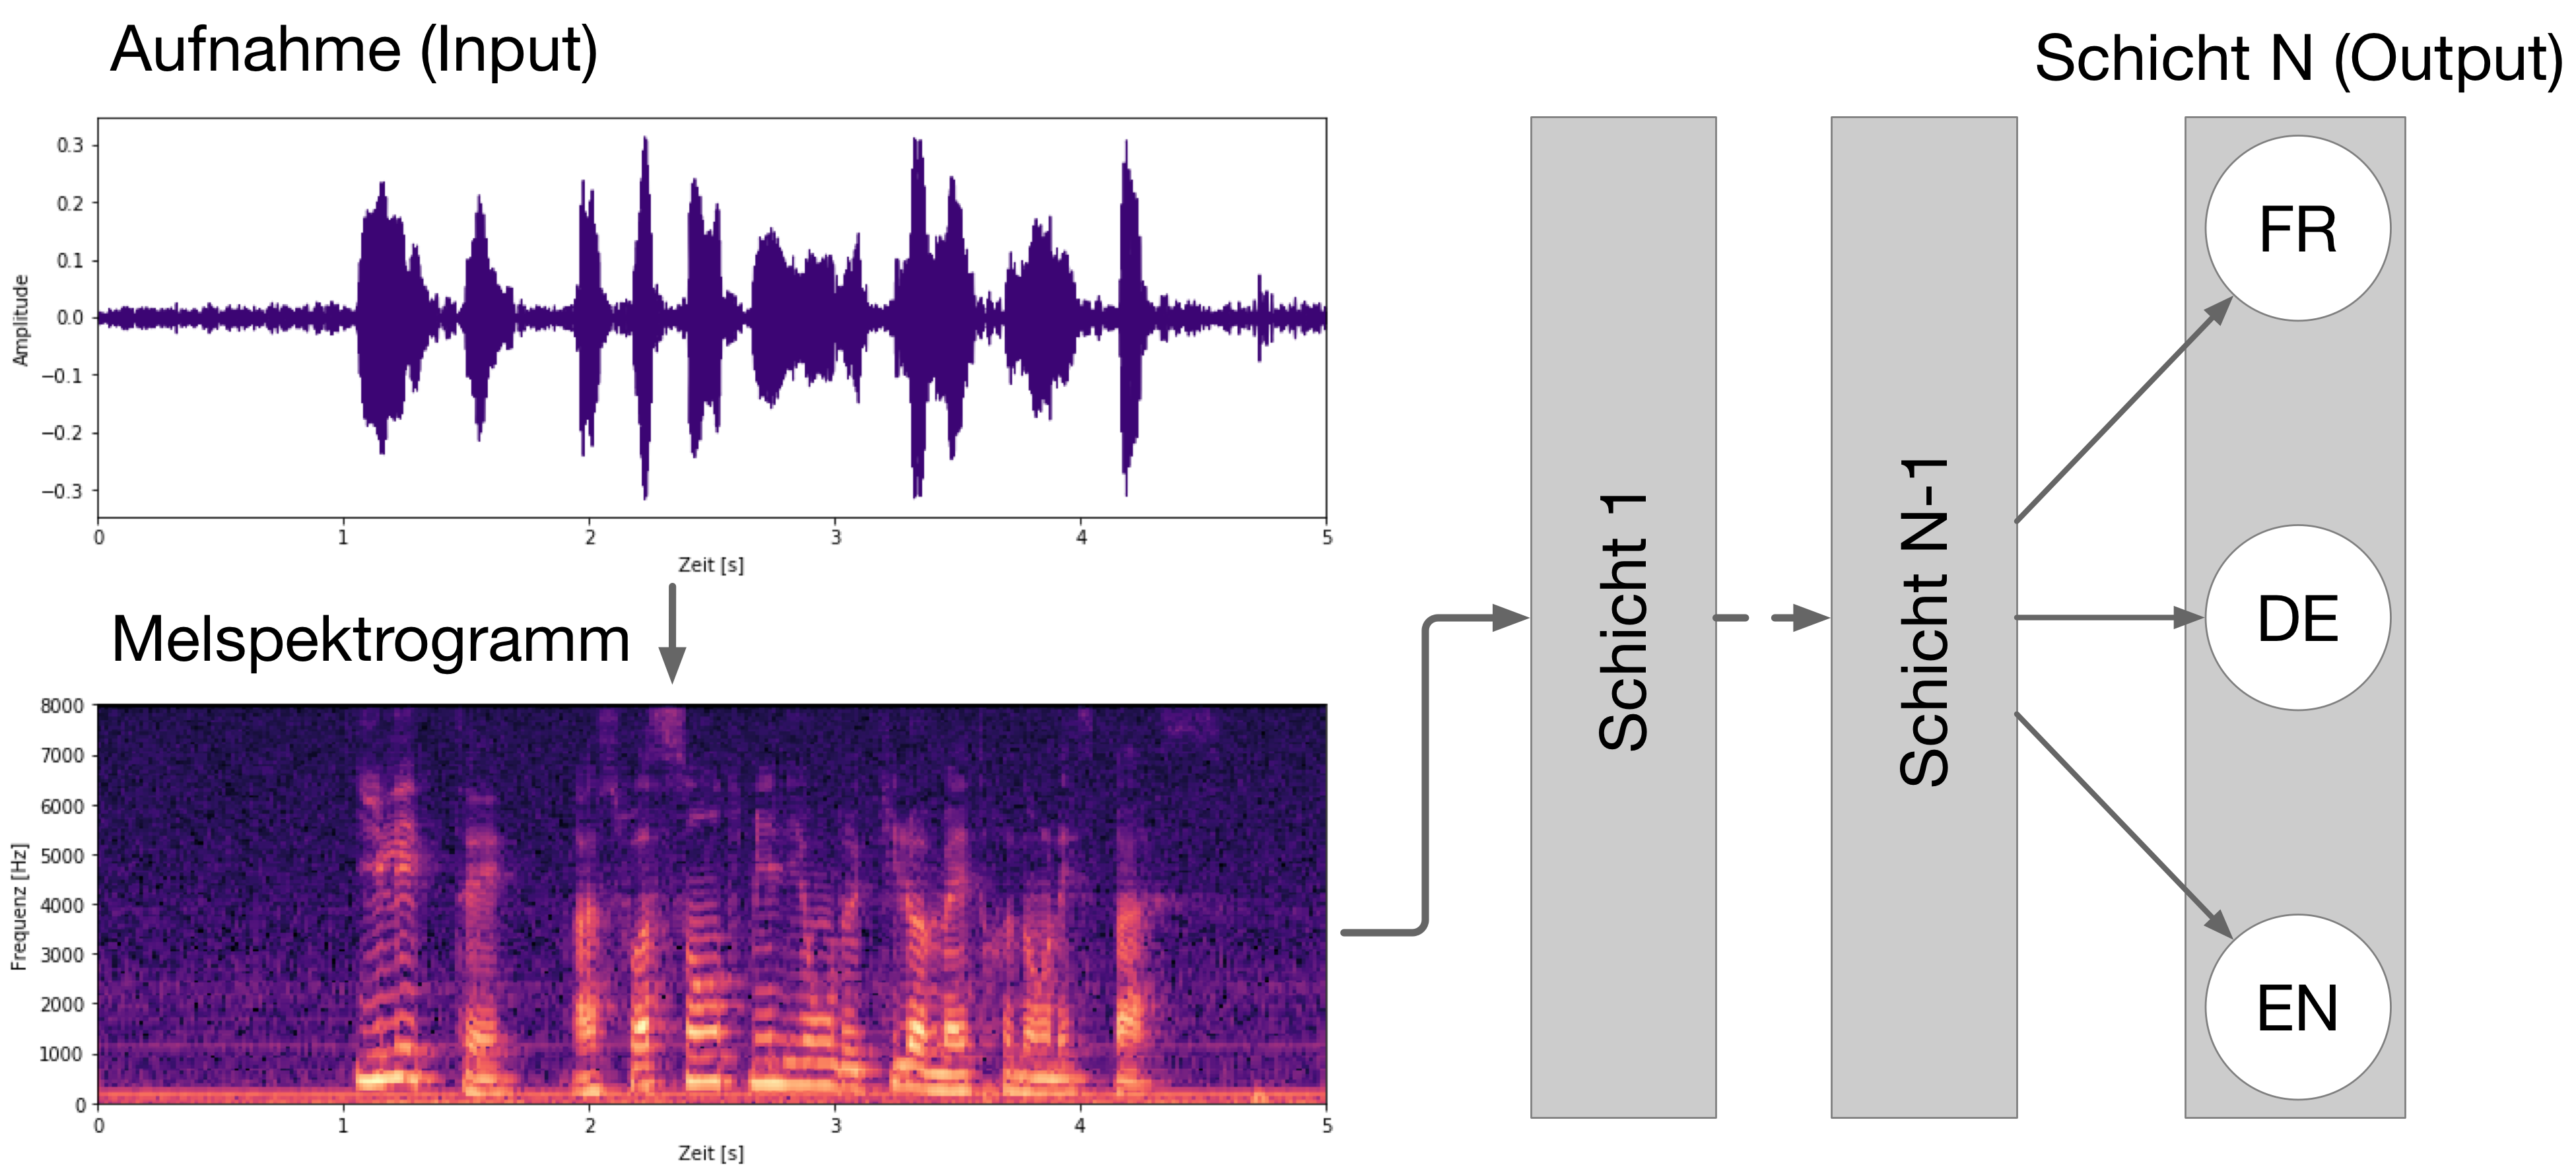
\includegraphics[width=0.8\textwidth]{assets/modelflow.png}
	\caption{Grundlegender Aufbau aller Modelle}
	\label{img:workflow}
\end{figure}


\subsection{CNN}
Das CNN Netzwerk akzeptiert Spektrogramme der Grösse 28x313, wobei 28 verschiedene Mel-Frequenzeimer berechnet werden an 313 Zeitpunkten. Das Netz besteht aus drei Convolution-MaxPooling Blocks und zwei Dense Schichten (Abbildung \ref{img:cnn}). Die Convolution-Grösse ist immer 3x3 und MaxPooling geschieht im Bereich 2x2. Die Anzahl Convolution's (Kanäle) nimmt von 64 auf 128 zu. 
\\
Die \textit{Fully Connected} Schicht besteht aus 512 Knoten mit 30\% \textit{Dropout}. Bei Dropout wird ein zufälliger gewählter Anteil der Eingabe der Schicht mit 0 ersetzt. Das Netz lernt dann, ohne diese Verbindungen auszukommen und somit mehrere Verbindungen einzelnen starken Verbindungen vorzuziehen. Die Eigenschaft hat einen positiven Einfluss auf die Robustheit des Netzes gegenüber neuen Daten \parencite[][Kap. 4.4.3]{chollet}.
\\
Die Architektur entspricht massgeblich der vorgestellten Architektur in \parencite{iLID} plus Dropout.
 \begin{figure}[hbt]
	\centering
		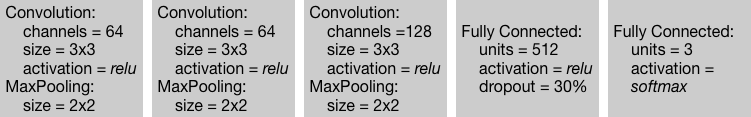
\includegraphics[width=0.8\textwidth]{assets/cnn.png}
	\caption{CNN Architektur}
	\label{img:cnn}
\end{figure}

\subsection{MobileNet-CNN}
Andere Arbeiten hatten gezeigt, dass grosse CNN Architekturen die auf dem \textit{ImageNet}\parencite{imagenet} Datenset (Riesiges Bilddatenset mit tausenden Bidklassen) stark sind, ebenfalls für Audioklassifizierung geignet sind \parencite{cnn_large}. Um Leistung zu sparen wurden Experimente mit \textit{MobileNet} durchgeführt.
MobileNet ist eine bekannte CNN Architektur entwickelt von \textit{Google} \parencite[][(V2)]{mobilenet}. Das Modell ist speziell entwickelt für Mobilgeräte, die in der Regel schwächere Hardware als Desktop-Computer besitzen. Das Ziel war ein effizientes Netzwerk für Bilderkennung im grossen Umfang, wie z.B ImageNet. Da das Modell in dieser Arbeit nur zwischen drei Klassen unterscheiden muss, wird die Anzahl Knoten im Netzwerk so weit wie möglich verkleinert, bzw. der Parameter $\alpha$ im Paper wird auf 0.25 gesetzt. 
\\
Das Netzwerk besitzt insgesamt 21 Schichten. Das Netzt funktioniert am bessten mit Eingaben der Grösse 224x224, der Bildgrösse in ImageNet. Die Spektrogramme werden darum auf dieses Format skaliert.
 \begin{figure}[hbt]
	\centering
		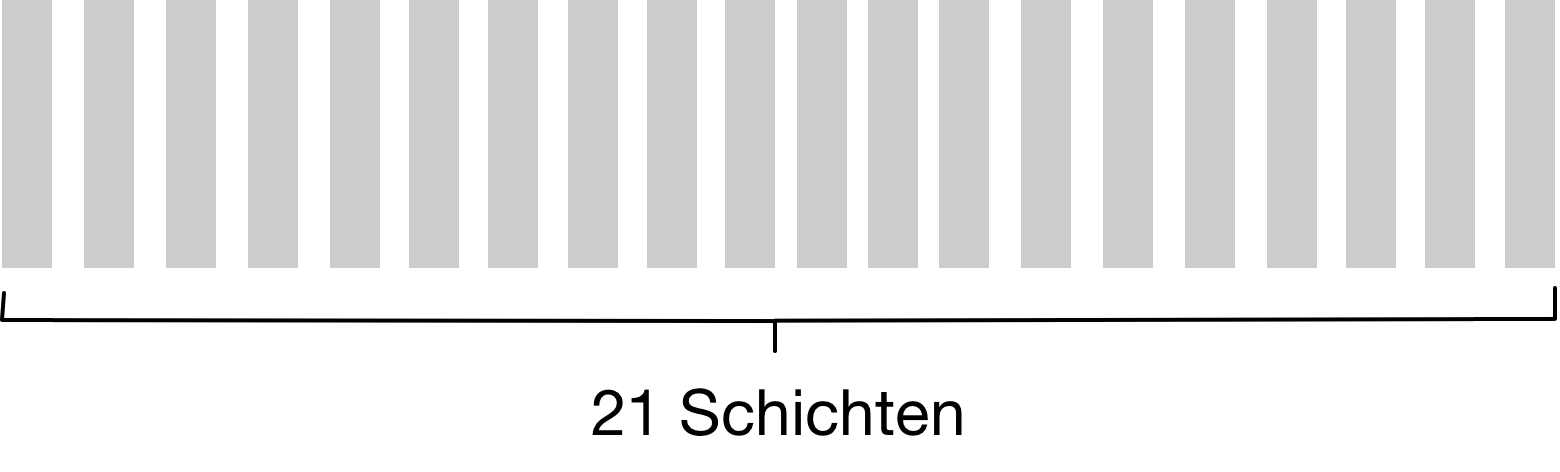
\includegraphics[width=0.8\textwidth]{assets/mobilenet.png}
	\caption{MobileNet Architektur}
	\label{img:mobilenet}
\end{figure}

\subsection{CRNN}
Convolutional Recurrent Neural Networks, eine Mischung aus CNN und RNN, wurden bereits erfolgreich auf Sprachidentifikation angewendet \parencite{crnn}\parencite{yerevann}. RNN's für Tonaufnahmen zu verwenden ist sinnvoll, denn Audiodaten sind naturgemäss zeitliche Folgen, also ideal für RNN's. RNN's haben aber den Nachteil, dass sie langsam lernen. Darum soll der CNN Teil im Vorfeld aus dem Spektrogramm eine kompaktere Repräsentation berechnet, z.b eine Abfolge von Phonemen. Da die Lernzeit proportional zur Eingabegrösse ist, lernt der RNN teil mit dieser Eingabe schneller. Es gibt keine Möglichkeit zu verifizieren, ob das CNN wirklich Phoneme berechnet aber die Resultate zeigen, dass das CRNN besser abschneidet als das CNN.
\\
Der CNN Teil besteht aus fünf Blocks von Convolution, MaxPooling und \textit{Batch Normalization}\label{Batch Normalization} (Siehe Abbildung \ref{img:crnn}). Die Idee von \textit{Batch Normalization} ist, dass die Ausgabe der vorherigen Schicht so normalisiert wird, dass sie den Durchschnitt 0 und die Varianz 1 besitzt. \textit{Batch Normalization} bringt den vor allem den Vorteil, dass das Modell schneller konvergiert, also schneller bessere Leistungen erbringt. \parencite{batch}
\\
Die Anzahl Convolutions steigert sich schrittweise von 16 auf 64. Das Convolution-Fenster hat immer die Grösse 4x4 und MaxPooling das Fenster 2x2. Bei den Convolutions wird 0.01 \textit{L2-Regularisation} verwendet:
$$ Verlust = Verlust + \sum_{i} w_{i}^{2}$$
Das bedeutet, dass dem Verlustwert zusätzlich das Quadrat der Gewichte addiert wird \parencite[Kap.~7.1.1]{goodfellow}. Übermässig hohe Gewichte werden überproportial gewertet. Die Regularisation hat das gleiche Ziel wie Dropout, das Netz robuster zu gestalten.
\\

 \begin{figure}[hbt]
	\centering
		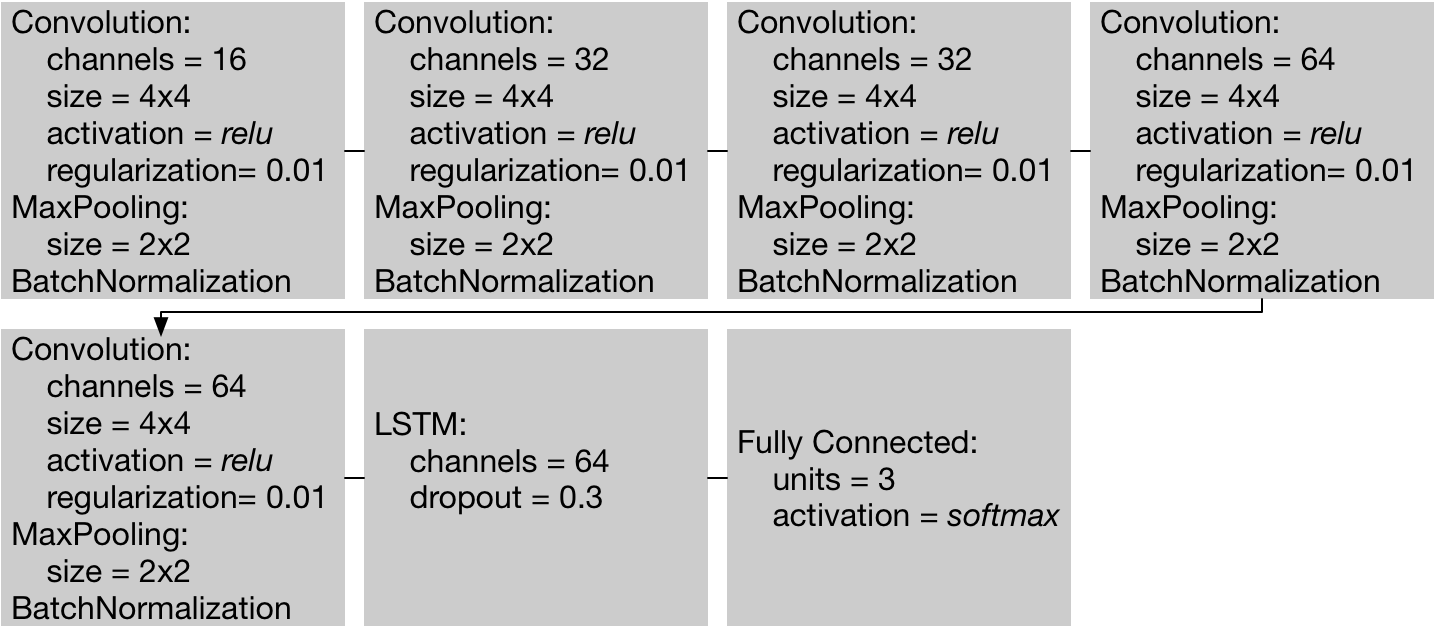
\includegraphics[width=0.8\textwidth]{assets/crnn.png}
	\caption{CRNN Architektur}
	\label{img:crnn}
\end{figure}

\section{Auswertung}

\subsection{Auswertung an Voxforge und YouTube}

\begin{table}[h]
	\centering
	\begin{tabular}{lllll}
		\hline
		Netz & Architektur     & Accuracy & MAE \\ \hline
		CNN  & 3 Conv          & 95.1\%     & 0.046  \\
		CRNN & 4 Conv + LSTM   & 96.2\%     & 0.031  \\
		CNN  & 28 Conv + Dense & 87\%     & 0.03  \\ \hline
	\end{tabular}
	\caption{Voxforge und YouTube Richtigkeit}
	\label{table:test}
\end{table}

\begin{table}[h]
	\centering
	\begin{tabular}{lll}
		\hline
		Netz & Trainingsdauer \\ \hline
		CNN  & 21 min \\
		CRNN & 68 min \\
		CNN  & 2h\\ \hline
	\end{tabular}
	\caption{Trainingsdauer}
	\label{table:test}
\end{table}

 \begin{figure}[hbt]
	\centering
		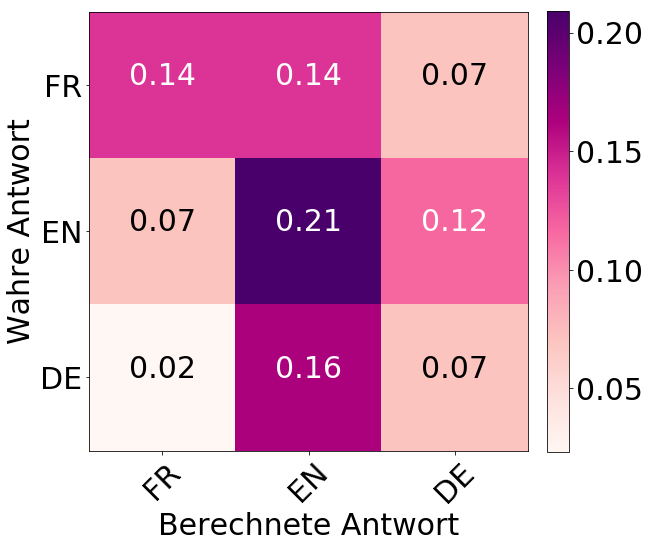
\includegraphics[width=0.5\textwidth]{assets/matrix.png}
	\caption{Normierte Wahrheitsmatrix}
	\label{img:matrix}
\end{figure}

\subsection{Auswertung an Librivox}
